\begin{figure}[t]
	\centering
	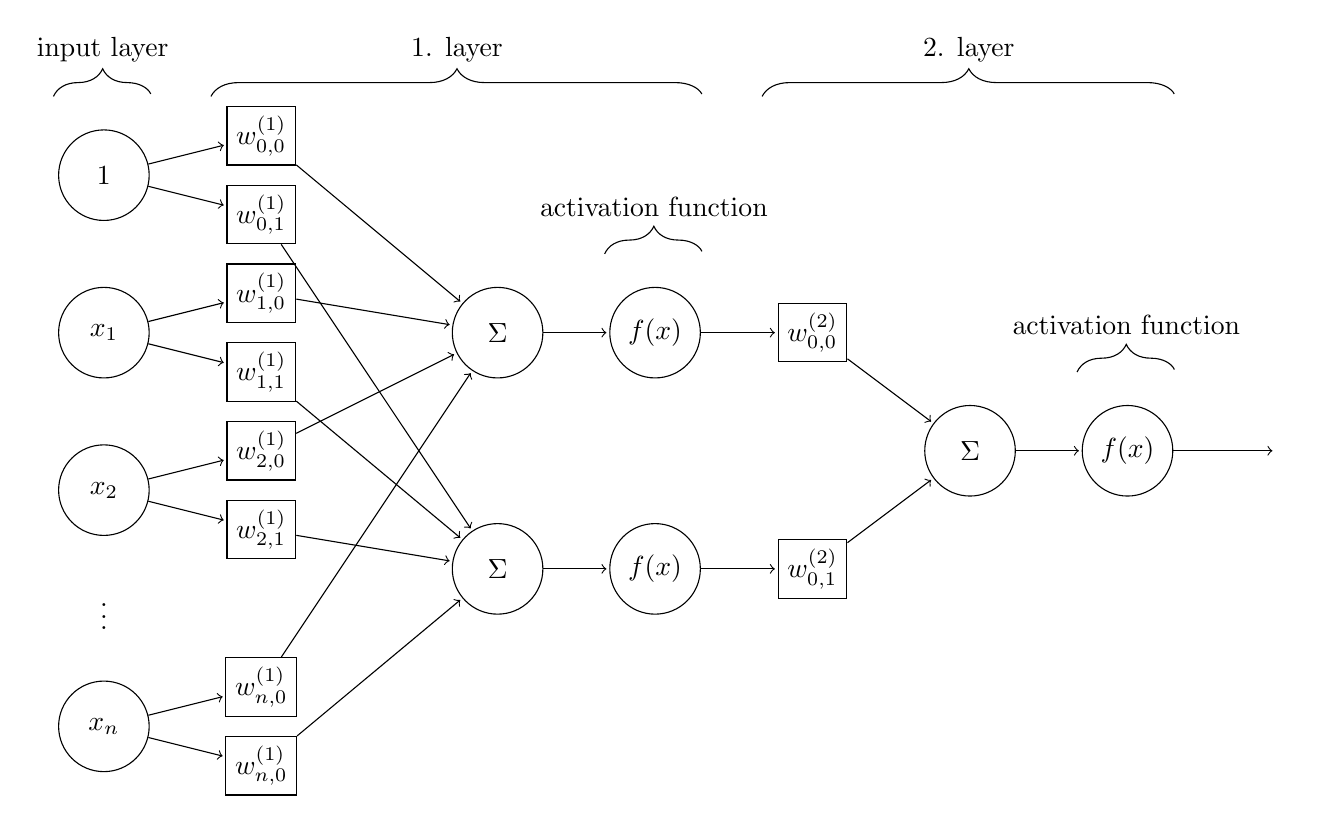
\begin{tikzpicture}[shorten >=1pt]
		\tikzstyle{unit}=[draw,shape=circle,minimum size=1.15cm]
		\tikzstyle{hidden}=[draw=none]
        \tikzstyle{weight}=[draw,shape=rectangle,minimum size=0.6cm]


        % input layer
        \node[unit](b0) at (0, 7, 0){$1$};
        \node[unit](x1) at (0, 5, 0){$x_1$};
        \node[unit](x2) at (0, 3, 0){$x_2$};
        \node at (0, 1.5){\vdots};
        \node[unit](xn) at (0, 0, 0){$x_n$};
		\draw [decorate,decoration={brace,amplitude=10pt},xshift=-4pt,yshift=0pt] (-0.5,8) -- (0.75,8) node [black,midway,yshift=+0.6cm]{input layer};

        % weight layer
        \node[weight](w00) at (2, 7.5, 0){$w^{(1)}_{0,0}$};
        \node[weight](w01) at (2, 6.5, 0){$w^{(1)}_{0,1}$};

        \node[weight](w10) at (2, 5.5, 0){$w^{(1)}_{1,0}$};
        \node[weight](w11) at (2, 4.5, 0){$w^{(1)}_{1,1}$};

        \node[weight](w20) at (2, 3.5, 0){$w^{(1)}_{2,0}$};
        \node[weight](w21) at (2, 2.5, 0){$w^{(1)}_{2,1}$};

        \node[weight](wn0) at (2, 0.5, 0){$w^{(1)}_{n,0}$};
        \node[weight](wn1) at (2, -0.5, 0){$w^{(1)}_{n,0}$};

        % sum layer
        \node[unit](sum0) at (5, 5, 0){$\Sigma$};
        \node[unit](sum1) at (5, 2, 0){$\Sigma$};

        % activation layer
        \node[unit](acti0) at (7, 5, 0){$f(x)$};
        \node[unit](acti1) at (7, 2, 0){$f(x)$};
		\draw [decorate,decoration={brace,amplitude=10pt},xshift=-4pt,yshift=0pt] (6.5,6) -- (7.75,6) node [black,midway,yshift=+0.6cm]{activation function};

		\draw [decorate,decoration={brace,amplitude=10pt},xshift=-4pt,yshift=0pt] (1.5,8) -- (7.75,8) node [black,midway,yshift=+0.6cm]{1. layer};

        % weight layer 2
        \node[weight](w200) at (9, 5, 0){$w^{(2)}_{0,0}$};
        \node[weight](w201) at (9, 2, 0){$w^{(2)}_{0,1}$};

        % sum layer 2
        \node[unit](sum2) at (11, 3.5, 0){$\Sigma$};

        % activation layer 2
        \node[unit](acti2) at (13, 3.5, 0){$f(x)$};
		\draw [decorate,decoration={brace,amplitude=10pt},xshift=-4pt,yshift=0pt] (12.5,4.5) -- (13.75,4.5) node [black,midway,yshift=+0.6cm]{activation function};


		\draw [decorate,decoration={brace,amplitude=10pt},xshift=-4pt,yshift=0pt] (8.5,8) -- (13.75,8) node [black,midway,yshift=+0.6cm]{2. layer};

        % hidden output
        \node[hidden](h0) at (15, 3.5, 0){};

        \draw[->](b0) -- (w00);
        \draw[->](b0) -- (w01);

        \draw[->](x1) -- (w10);
        \draw[->](x1) -- (w11);

        \draw[->](x2) -- (w20);
        \draw[->](x2) -- (w21);

        \draw[->](xn) -- (wn0);
        \draw[->](xn) -- (wn1);

        \draw[->](w00) -- (sum0);
        \draw[->](w10) -- (sum0);
        \draw[->](w20) -- (sum0);
        \draw[->](wn0) -- (sum0);

        \draw[->](w01) -- (sum1);
        \draw[->](w11) -- (sum1);
        \draw[->](w21) -- (sum1);
        \draw[->](wn1) -- (sum1);

        \draw[->](sum0) -- (acti0);
        \draw[->](sum1) -- (acti1);

        \draw[->](acti0) -- (w200);
        \draw[->](acti1) -- (w201);

        \draw[->](w200) -- (sum2);
        \draw[->](w201) -- (sum2);

        \draw[->](sum2) -- (acti2);
        \draw[->](acti2) -- (h0);

	\end{tikzpicture}
	\caption{A MLP with two hidden layers (two neurons in the first and one in the last), each input gets multiplied with each weight of each neuron, summed up and fed into an activation function to produce the input for the next layer, where this process is repeated.}
	\label{fig:mlp}
\end{figure}
